\documentclass[10pt]{beamer}

\usetheme[progressbar=frametitle]{metropolis}
\usepackage{appendixnumberbeamer}
\usepackage{listings}
\usepackage{graphicx,subfigure}
\usepackage[utf8]{inputenc}
\usepackage{eurosym}

\usepackage{booktabs}
\usepackage[scale=2]{ccicons}
\setbeamertemplate{caption}{\raggedright\insertcaption\par}

\usepackage{pgfplots}
\usepgfplotslibrary{dateplot}

\usepackage{xspace}
\newcommand{\themename}{\textbf{\textsc{metropolis}}\xspace}

\title{Alcaudon}
\subtitle{Streaming data platform}
% \date{\today}
\date{\today}
\author{Francisco Fernández Castaño}
\institute{Escuela Superior Informática - UCLM}
% \titlegraphic{\hfill\includegraphics[height=1.5cm]{logo.pdf}}

\begin{document}
\defverbatim[colored]\computationapi{%
\begin{lstlisting}[language=scala, captionpos=b, caption = {Computation API's}]
trait Computation
    extends ProduceAPI
    with TimerAPI
    with StateAPI
    with SerializationAPI
    with RuntimeContext {
  ...
  def processRecord(record: Record): Unit
  def processTimer(timer: Timer): Unit
  ...
}
\end{lstlisting}
}

\defverbatim[colored]\tx{%
  \begin{lstlisting}[language=scala, captionpos=b, caption = {Computation state persistence}]
case _: ComputationFinished =>
persist(Transaction(pendingChanges)) { transaction =>
  applyTx(transaction, origin)
  context.become(receiveCommand)
  cuckooFilter.put(runningRecordId)
  state.newProcessedRecord()
  clearPendingChanges()
  origin ! ACK(self, runningRecordId, 0l)
}
  \end{lstlisting}
}


\defverbatim[colored]\serializationapi{%
\begin{lstlisting}[language=scala, captionpos=b, caption = {Serializer-Deserializer typeclass}]
trait TypeInfo[T] {
  def serialize(obj: T)
               (implicit output: DataOutput)
               :DataOutput
  def deserialize(t: DataInput): T
}
\end{lstlisting}
}


\defverbatim[colored]\ride{%
\begin{lstlisting}[language=scala]
class RidePassengerCountComputation extends Computation {
  def processRecord(record: Record): Unit = {
    val ride: Ride = deserialize(record.value)
    val count = get(record.key) + ride.passengerCount
    if (count > settings.alertPassengers)
    produceRecord(alertSink,
                  RawRecord(serialize(record.key),
                            record.timestamp))
    set(count + ride.passengerCount)
    setTimer(FixedRecurrentTimer(cell, 5.minutes))
  }

\end{lstlisting}
}

\defverbatim[colored]\ridee{%
\begin{lstlisting}[language=scala]
  def processTimer(timeStamp: Timer): Unit = {
    val location = Utils.cellToLocation(timer.tag)
    val totalPassengerCount = get(timer.tag)
    val totalPassengers = RawRecord(serialize((location, totalPassengerCount))
    produceRecord(elasticSink,
                  totalPassengers,
                  record.timestamp))
  }
}
\end{lstlisting}
}


\defverbatim[colored]\ridedataflow{%
\begin{lstlisting}[language=scala]
val dataflow = DataflowBuilder("ridesCounter")
  .withSource("taxiRides", TaxiRides())
  .withComputation("filterNYRides",
    FilterRideComputation,
    OutputStreams("nycRides"),
    AlcaudonInputStream("taxiRides")
  .withComputation("passengerCount",
    RidePassengerCountComputation,
    OutputStreams("elasticSink", "alertSink"),
    AlcaudonInputStream("nycRides",
                        new RideKeyExtractor())
  .withSink("elasticSink", ElasticSearchSink)
  .withSink("alertSink",
            HTTPSink(settings.alertEndpoint))
  .build()
\end{lstlisting}
}

\maketitle

\begin{frame}{Table of contents}
  \setbeamertemplate{section in toc}[sections numbered]
  \tableofcontents[hideallsubsections]
\end{frame}

\section{Introduction}

\begin{frame}[fragile]{Introduction}
\begin{figure}[!h]
\begin{center}
\includegraphics[width=0.8\textwidth]{../figures/ciscodata.png}
\caption{Actual data stored in data centers}
\label{fig:ciscodata}
\end{center}
\end{figure}

  \end{frame}


\section{Objectives}

\begin{frame}{Objectives}
  \metroset{block=fill}

  \begin{block}{Alcaudon}
    The purpose of this project is to develop a distributed, fault-tolerant and
    elastic streaming processing framework aimed for unbounded datasets.
  \end{block}
\end{frame}


%% \begin{frame}{Specific objectives}
%%   \begin{itemize}
%%   \item Provide an abstraction to create distributed computations
%%   \item Develop mechanisms to ensure exactly-once processing of records
%%   \item Provide tools to work with out-of-order data
%%   \item Implement a cluster scheduler
%%   \item Allow extensibility of sources and sinks
%%   \item Design and implement an elastic, fault-tolerant and scalable distributed architecture
%%   \end{itemize}
%% \end{frame}

\section{State of the art}

\begin{frame}{State of the art}
\begin{figure}[!h]
\begin{center}
\includegraphics[width=1\textwidth]{../figures/mindmap.pdf}
\caption{Alcaudon foundations}
\label{fig:mindmap}
\end{center}
\end{figure}
  \end{frame}

\subsection{Data processing}

\begin{frame}[fragile]{Data processing}

  \begin{itemize}
  \item Data analysis as competitive advantage
  \item RDBMS cannot cope with large amounts of data
  \item HPC are not suitable for dynamic workloads
  \item Map-Reduce based systems
  \item Latency may be unacceptable in some scenarios
  \end{itemize}
\end{frame}


\begin{frame}{Streaming}
  Streaming characterization:
\textit{
\begin{itemize}
\item The data elements in the stream arrive online.
\item The system has no control over the order in which data elements arrive to
  be processed, either within a data stream or across data streams.
\item Data streams are potentially unbounded in size.
\item Once an element from a data stream has been processed it is discarded or
  archived — it cannot be retrieved easily unless it is explicitly stored in
  memory, which typically is small relative to the size of the data streams
\end{itemize}
}
  \end{frame}

\begin{frame}[fragile]{Cloud Computing}
  \begin{figure}[!h]
    \begin{center}
      \includegraphics[width=1\textwidth]{../figures/cloud.jpg}
    \end{center}
  \end{figure}
\end{frame}

\subsection{Distributed systems}

\begin{frame}[fragile]{Distributed systems}

  \begin{figure}[!h]
    \begin{center}
      \includegraphics[width=1\textwidth]{../figures/letter.jpg}
    \end{center}
  \end{figure}
  %% MAYBE USE AN IMAGE
  %% \begin{block}{Definition}
  %%   Distributed systems can be defined as a set of computer programs,
  %%   executing on one or more computers, and coordinating actions by
  %%   exchanging \textit{messages}~\cite{GuideReliable}. Those computers are
  %%   usually located in a \textit{computer network}, a collection of
  %%   computers interconnected by hardware that supports message passing and
  %%   implement routing protocols.
  %% \end{block}
\end{frame}


\begin{frame}[fragile]{Benefits of distributed systems}
  Scalability
  \begin{itemize}
  \item Reliability
  \item Elasticity
  \item Parallelism
  \item Price/performance ratio
  \end{itemize}
\end{frame}

\begin{frame}[fragile]{Challenges in distributed systems}
  \begin{columns}[T]
    \begin{column}{.4\textwidth}
      \begin{block}{}
        \begin{itemize}
        \item Notion of time
        \item Distributed state
        \item Membership protocols
        \end{itemize}
      \end{block}
    \end{column}
    \begin{column}{.6\textwidth}
      \begin{block}{}
        \includegraphics[width=1\textwidth]{../figures/clocks.jpg}
      \end{block}
    \end{column}
  \end{columns}
\end{frame}

\subsection{Job scheduling}

\begin{frame}{Job scheduling}
  \begin{figure}[!h]
    \centering
    \includegraphics[width=0.6\textwidth]{../figures/jssp.png}
    \label{fig:jssp}
  \end{figure}
  NP-Hard problem
\end{frame}

\subsection{Library design}
\begin{frame}{Library design}
  \begin{figure}[!h]
    \centering
    \includegraphics[width=1\textwidth]{../figures/abstraction.jpg}
    \label{fig:jssp}
  \end{figure}
\end{frame}

\section{Methodology}

\begin{frame}{Methodology}
  \begin{figure}
    \centering
    \includegraphics[width=0.6\textwidth]{../figures/xp.png}
    \caption{Extreme Programming feedback diagram}
    \label{fig:xp}
  \end{figure}
  15 iterative releases
\end{frame}

\begin{frame}{Methodology}
  \begin{itemize}
  \item Continuous integration (Travis CI)
  \item Continuous deployment (Maven central and Docker Hub)
  \end{itemize}
\end{frame}

\begin{frame}{Costs}
  \begin{table}[hp]
    \centering
    \begin{tabular}{|l|c|r|}
      \hline
      \textbf{Resource} & \textbf{Quantity} & \textbf{Cost} \\ \hline
      \begin{tabular}[c]{@{}l@{}}Distributed systems developer\end{tabular}  & 1 & \EUR{50000} \\ \hline
        \begin{tabular}[c]{@{}l@{}}Dell XPS 13\end{tabular} & 1 & \EUR{1500} \\ \hline
          \begin{tabular}[c]{@{}l@{}}AWS EC2 instance hour\end{tabular} & 100 hours & \EUR{50} \\ \hline \hline
            \begin{tabular}[c]{@{}l@{}}Total:\end{tabular} &  & \EUR{51550} \\ \hline
    \end{tabular}
  \end{table}
\end{frame}

\section{Architecture}

\begin{frame}[fragile]{General overview}
\begin{figure}[!h]
  \centering
  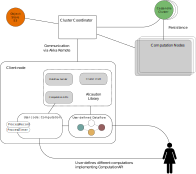
\includegraphics[width=0.8\textwidth]{../figures/architecture-mini.pdf}
  \label{fig:architecture}
\end{figure}
\end{frame}

\begin{frame}[fragile]{Alcaudon library}
\begin{figure}[!h]
  \centering
  \includegraphics[width=0.6\textwidth]{../figures/client.pdf}
  \caption{Alcaudon library}
  \label{fig:library}
\end{figure}
\end{frame}


\begin{frame}[fragile]{Computation APIs}
\begin{figure}[!h]
  \centering
  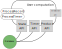
\includegraphics[width=0.5\textwidth]{../figures/libraryApi.pdf}
  \caption{Alcaudon computation API's}
  \label{fig:apis}
\end{figure}
\end{frame}


\begin{frame}[fragile]{Computation APIs}
\computationapi
\end{frame}

\begin{frame}[fragile]{Dataflow builder}
\begin{figure}
  \centering
  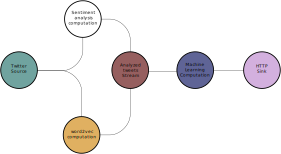
\includegraphics[width=0.8\textwidth]{../figures/dataflowbuilder.pdf}
  \caption{Dataflow DAG example}
  \label{fig:dataflowbuilder}
\end{figure}
\end{frame}

\begin{frame}[fragile]{Serialization API}
  \serializationapi
\end{frame}

\subsection{Computation node}

\begin{frame}[fragile]{Computation node}
\begin{figure}[!h]
  \centering
  \includegraphics[width=0.5\textwidth]{../figures/computationnode.pdf}
  \caption{Computation node modules}
  \label{fig:computationnode}
\end{figure}
\end{frame}


%% \begin{frame}[fragile]{Cluster membership}
%%   \begin{figure}[!h]
%%     \begin{center}
%%       \includegraphics[width=0.6\textwidth]{../figures/membershipcluster.png}
%%       \caption{Akka cluster membership states~\cite{akkastates}}
%%       \label{fig:statescluster}
%%     \end{center}
%%   \end{figure}

%%   Module in charge of managing node lifecycle
%% \end{frame}

\begin{frame}[fragile]{Computation manager}
  Module in charge of deploying user code.
  \begin{itemize}
  \item ComputationExecutor and Stream actors are deployed
  \item Logical addresses are disseminated via CRDT's
  \item Coordinator is acknowledged
  \end{itemize}
\end{frame}

\begin{frame}[fragile]{Computation executor}
  Component in charge of executing user code.
  \begin{enumerate}
  \item Using duplication detection logic, records are checked to avoid duplicates.
  \item User defined code is run for the received record. This execution can
    result in pending changes to timers, state or downstream productions.
  \item Pending changes are saved into the database.
  \item An acknowledgment is sent back to senders.
  \item Pending new records are sent.
  \end{enumerate}
\end{frame}


\begin{frame}[fragile]{Computation executor}
\tx
\end{frame}

\begin{frame}[fragile]{Timers implementation}
  \begin{itemize}
  \item \textit{Fixed timers}
  \item \textit{Recurrent fixed timers}
  \item \textit{Watermark timers}
  \end{itemize}
\end{frame}

\begin{frame}[fragile]{Timers}
\begin{figure}
\centering
\begin{subfigure}
  \centering
  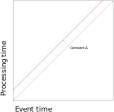
\includegraphics[width=0.4\linewidth]{../figures/constantskew.pdf}
\end{subfigure}%
\begin{subfigure}
  \centering
  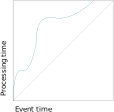
\includegraphics[width=0.4\linewidth]{../figures/realskew.pdf}
\end{subfigure}
\caption{Differences between ideal event time-process time skew and real world skew}
\label{fig:skew}
\end{figure}
\end{frame}

\begin{frame}[fragile]{Timers implementation}
  \begin{definition}{Watermark:}
    Given a computation, $A$, let the oldest processed record in $A$ be a timestamp
    corresponding to the oldest unfinished record in $A$.
    Given this, watermark of $A$ is:
    $min($oldest record of $A$, watermark of $C$ : $A$ depends on C$)$.
  \end{definition}
  Implemented using CRDT's
\end{frame}

\begin{frame}[fragile]{Streams}
  \metroset{block=fill}
  \begin{block}{Streams}
    In Alcaudon, streams represent the delivery instrument between different
    computations.
  \end{block}

  Hybrid flow control
\end{frame}

\begin{frame}[fragile]{Coordinator node}
  \begin{figure}[!h]
    \centering
    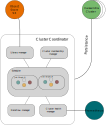
\includegraphics[width=0.5\textwidth]{../figures/coordinator.pdf}
    \caption{Coordinator node modules}
    \label{fig:coordinatormodules}
  \end{figure}
\end{frame}


\begin{frame}[fragile]{Scheduling}
  \begin{figure}[!h]
    \centering
    
\includegraphics[width=0.8\textwidth]{../figures/scheduling.pdf}
    \caption{Scheduling process}
    \label{fig:scheduler}
  \end{figure}
  Alcaudon uses a state-of-the-art cluster scheduler platform,
  named \alert{Firmament}.
\end{frame}

\begin{frame}[fragile]{Scheduling}

  \begin{itemize}
  \item \textit{Trivial}: Fixed costs, tasks always schedule if resources are idle.
  \item \textit{Random}: Random costs, for fuzz tests.
  \item \textit{SJF}: Shortest job first policy based on average past runtimes.
  \item \textit{Quincy}: Original Quincy cost model, with data locality.
  \item \textit{Whare}: Implementation of Whare-Map's M and MCs policies.
  \item \textit{\alert{CoCo}}: Coordinated co-location model.
  \item \textit{Octopus}: Simple load balancing based on task counts.
  \item \textit{Void}: Bogus cost model used for KB with simple scheduler.
  \item \textit{NET-BW}: Network-bandwidth-aware cost model (avoids hotspots).
  \end{itemize}
\end{frame}

\section{Results}

\begin{frame}[fragile]{Demo}
A public\footnote{http://www.nyc.gov/html/tlc} data set of the New York City
Taxi and Limousine Commission (TLC) will be used.

A dataflow pipeline will be programmed in order to find popular spots in NYC.
\end{frame}


\begin{frame}[fragile]{Demo}
  Demo video
\end{frame}


\begin{frame}[fragile]{Achieved Results}
  \begin{itemize}
    \item Provide an abstraction to create distributed computations
    \item Develop mechanisms to ensure exactly-once processing of records
    \item Provide tools to work with out-of-order data
    \item Implement a cluster scheduler
    \item Allow extensibility of sources and sinks
    \item Design and implement an elastic, fault-tolerant and scalable distributed architecture
  \end{itemize}
\end{frame}

\begin{frame}{Additional materials}
  In the manuscript there are more materials described and given the lack of
  time they have not been presented.
\end{frame}

\section{Questions}

%%   Get the source of this theme and the demo presentation from

%%   \begin{center}\url{github.com/matze/mtheme}\end{center}

%%   The theme \emph{itself} is licensed under a
%%   \href{http://creativecommons.org/licenses/by-sa/4.0/}{Creative Commons
%%   Attribution-ShareAlike 4.0 International License}.

%%   \begin{center}\ccbysa\end{center}

%% \end{frame}

%% {\setbeamercolor{palette primary}{fg=black, bg=yellow}
%% \begin{frame}[standout]
%%   Questions?
%% \end{frame}
%% }

\appendix


\begin{frame}[fragile]{Demo}
\ride
\end{frame}


\begin{frame}[fragile]{Demo}
\ridee
\end{frame}


\begin{frame}[fragile]{Demo}
\ridedataflow
\end{frame}

%% \begin{frame}[fragile]{Backup slides}
%%   Sometimes, it is useful to add slides at the end of your presentation to
%%   refer to during audience questions.

%%   The best way to do this is to include the \verb|appendixnumberbeamer|
%%   package in your preamble and call \verb|\appendix| before your backup slides.

%%   \themename will automatically turn off slide numbering and progress bars for
%%   slides in the appendix.
%% \end{frame}

%% \begin{frame}[allowframebreaks]{References}

%%   \bibliography{demo}
%%   \bibliographystyle{abbrv}

%% \end{frame}

\end{document}

